% ==============================================================
% 09_presentation.tex
% "Money and Success in Football: Does Financial Strength
%  Predict League Position?"
% Beamer / Metropolis — compile with: xelatex deliverables/09_presentation.tex
% (run from project root so \graphicspath{{outputs/}} resolves)
% Submission: July 2, 2026 | Presentation: July 8, 2026
% ==============================================================
\documentclass[aspectratio=1610,10pt]{beamer}

% ── Metropolis theme ──────────────────────────────────────────
\usetheme[progressbar=frametitle, block=fill, numbering=fraction]{metropolis}

% ── xelatex font setup ───────────────────────────────────────
\usepackage{fontspec}
\usepackage{microtype}

% ── Core packages ─────────────────────────────────────────────
\usepackage{graphicx}
\usepackage{booktabs}
\usepackage{colortbl}
\usepackage{xcolor}
\usepackage{tikz}
\usepackage{array}
\usepackage{amsmath}
\usepackage{url}
\usepackage{calc}

% ── Image path (compile from project root) ────────────────────
\graphicspath{{outputs/}}

% ── Project colour palette ────────────────────────────────────
\definecolor{NavyBlue}{HTML}{1A2A4A}
\definecolor{PitchGold}{HTML}{F5A623}
\definecolor{AlertRed}{HTML}{C0392B}
\definecolor{GrassGreen}{HTML}{196F3D}
\definecolor{SteelBlue}{HTML}{2C3E73}
\definecolor{SlateGrey}{HTML}{566573}
\definecolor{RowA}{HTML}{EBF5FB}
\definecolor{RowB}{HTML}{FEF9E7}
\definecolor{LightRed}{HTML}{FDEDEC}

% ── Metropolis colour overrides ───────────────────────────────
\setbeamercolor{normal text}{fg=NavyBlue, bg=white}
\setbeamercolor{frametitle}{bg=NavyBlue, fg=white}
\setbeamercolor{title separator}{fg=PitchGold}
\setbeamercolor{progress bar}{fg=PitchGold, bg=NavyBlue!25}
\setbeamercolor{progress bar in section page}{fg=PitchGold, bg=NavyBlue!25}
\setbeamercolor{alerted text}{fg=AlertRed}
\setbeamercolor{example text}{fg=GrassGreen}
\setbeamercolor{block title}{bg=NavyBlue!12, fg=NavyBlue}
\setbeamercolor{block body}{bg=NavyBlue!5, fg=NavyBlue}
\setbeamercolor{block title alerted}{bg=AlertRed!12, fg=AlertRed}
\setbeamercolor{block body alerted}{bg=AlertRed!5}
\setbeamercolor{block title example}{bg=GrassGreen!12, fg=GrassGreen}
\setbeamercolor{block body example}{bg=GrassGreen!5}

\metroset{titleformat=smallcaps}

% ── TU Dortmund logo (conditional on file presence) ───────────
% Place tu-do-logo.pdf next to this .tex file or in the project root.
\IfFileExists{tu-do-logo.pdf}{%
  \titlegraphic{\hfill\includegraphics[height=1.0cm]{tu-do-logo.pdf}}%
  %%\logo{\includegraphics[height=0.55cm]{tu-do-logo.pdf}}%
}{\titlegraphic{}\logo{}}

% ── Presentation metadata ─────────────────────────────────────
\title{Money and Success in Football}
\subtitle{Does Financial Strength Predict League Titles?}
\author[Group X]{%
  \texorpdfstring{%
    {\small\textbf{Group X:}\\[0.2em]
    Md Muktadir \quad|\quad Linus Mainka}%
  }{Group X}}
\institute{\small TU Dortmund University
  \textendash{} Department of Statistics}
\date{\small Summer Semester 2026 \quad|\quad
  Final Presentation \quad|\quad 08 July 2026}

% ── Callout box commands (consistent with 08_final_presentation) ─
\newcommand{\findingbox}[1]{%
  \begin{tikzpicture}
    \node[fill=PitchGold!18, draw=PitchGold, line width=0.9pt,
          rounded corners=4pt, inner sep=9pt,
          text width=\linewidth-10pt]%
      {\small\bfseries\color{NavyBlue}#1};
  \end{tikzpicture}}

\newcommand{\alertbox}[1]{%
  \begin{tikzpicture}
    \node[fill=AlertRed!10, draw=AlertRed, line width=0.9pt,
          rounded corners=4pt, inner sep=9pt,
          text width=\linewidth-10pt]%
      {\small\bfseries\color{AlertRed}#1};
  \end{tikzpicture}}

\newcommand{\statpanel}[2]{%
  \begin{tikzpicture}
    \node[fill=NavyBlue!7, draw=NavyBlue!25, line width=0.6pt,
          rounded corners=4pt, inner sep=9pt,
          text width=\linewidth-10pt, align=center]%
      {{\large\bfseries\color{NavyBlue}#1}\par\smallskip
       {\footnotesize\color{SlateGrey}#2}};
  \end{tikzpicture}}

\newcommand{\duallabel}[2]{%
  \begin{tikzpicture}
    \node[fill=RowA, draw=SteelBlue!30, line width=0.5pt,
          rounded corners=3pt, inner sep=8pt,
          text width=\linewidth-10pt]%
      {{\footnotesize\textbf{\color{SteelBlue}Statistical:}~#1}%
       \par\smallskip
       {\footnotesize\textbf{\color{GrassGreen}Plain English:}~#2}};
  \end{tikzpicture}}

% ─────────────────────────────────────────────────────────────
\begin{document}

% ══════════════════════════════════════════════════════════════
% SLIDE 1 — Title
% ══════════════════════════════════════════════════════════════
\maketitle

% ══════════════════════════════════════════════════════════════
% SLIDE 2 — Research Question and Motivation
% ══════════════════════════════════════════════════════════════
\begin{frame}[shrink=8]{Does Financial Strength Predict League Position?}
  \vspace{2pt}
  {\normalsize\color{NavyBlue}%
   \textbf{Research Question:} Does a squad's financial rank within its league
   systematically determine where it finishes in the final standings?}
  \vspace{8pt}

  \begin{columns}[T]
    \begin{column}{0.53\textwidth}
      \textbf{Why this matters:}
      \begin{itemize}\setlength\itemsep{6pt}
        \item Europe's five major leagues generate over
              \textbf{\texteuro{}18 billion} in annual revenue;
              transfer spending exceeded \textbf{\texteuro{}12 billion}
              in 2023--24 alone.
        \item UEFA introduced \textbf{Financial Fair Play} precisely
              to limit financial dominance --- implying money
              \emph{does} buy success.
        \item If outcomes are financially predetermined, competitive
              drama is fundamentally reduced for fans of smaller clubs.
      \end{itemize}
    \end{column}
    \begin{column}{0.43\textwidth}
      \vspace{4pt}
      \findingbox{This study uses \textbf{976 team-seasons} from
        5 leagues and 10 seasons (2015--16 to 2024--25)
        to answer with evidence, not opinion.}
      \vspace{8pt}
      {\small\color{SlateGrey}
        Two contrasting cases --- one financially expected,
        one statistically miraculous --- motivate why the
        question requires careful empirical investigation.}
    \end{column}
  \end{columns}
\end{frame}

% ══════════════════════════════════════════════════════════════
% SLIDE 3 — Two Motivating Cases
% ══════════════════════════════════════════════════════════════
\begin{frame}[shrink=8]{Two Cases: One Expected, One Miraculous}
  \begin{columns}[T]
    \begin{column}{0.47\textwidth}
      \begin{alertblock}{Leicester City 2015--16}
        {\small
        \begin{tabular}{@{}l l@{}}
          Financial Rank   & \textbf{11th} of 20 \\
          League           & Premier League \\
          Squad value      & \textsterling{}161M
                             (avg: \textsterling{}458M) \\
          Model prediction & 11.5th place \\
          Actual finish    & \textbf{1st (Champion)} \\
          Residual         & $\mathbf{-10.5}$ positions \\
          Bookmaker odds   & \textbf{5\,000-to-1} \\
        \end{tabular}
        \par\vspace{5pt}
        The largest single-season overperformance in the
        entire 10-year dataset --- a statistical shock that
        occurs with probability well below 0.1\%.}
      \end{alertblock}
    \end{column}
    \begin{column}{0.47\textwidth}
      \begin{exampleblock}{Bayer Leverkusen 2023--24}
        {\small
        \begin{tabular}{@{}l l@{}}
          Financial Rank & \textbf{2nd} (Bundesliga) \\
          Result         & \textbf{Bundesliga champions} \\
          Historic feat  & First unbeaten Bundesliga season \\
          Context        & Ended Bayern's 11-year streak \\
          Residual       & $-1.8$ (within normal range) \\
        \end{tabular}
        \par\vspace{5pt}
        Remarkable by football standards, but
        statistically \emph{expected}: the
        second-richest squad winning is precisely what
        the financial hierarchy predicts.}
      \end{exampleblock}
    \end{column}
  \end{columns}
  \vspace{10pt}
  \findingbox{These two cases bracket the full spectrum of outcomes:
    from the financially-expected champion to the greatest financial
    upset in modern football.}
\end{frame}

% ══════════════════════════════════════════════════════════════
% SLIDE 4 — Data and Scope
% ══════════════════════════════════════════════════════════════
\begin{frame}[shrink=8]{Data and Scope: 976 Team-Seasons Across Five Leagues}
  \begin{columns}[T]
    \begin{column}{0.50\textwidth}
      \vspace{2pt}
      \textbf{Two data sources:}
      \begin{itemize}\setlength\itemsep{4pt}
        \item \textbf{ESPN FC} --- final league standings, all five leagues,
              seasons 2015--16 through 2024--25.
        \item \textbf{Transfermarkt} --- squad total market value
              (\texteuro{}M) at the start of each season.
      \end{itemize}
      \vspace{6pt}
      {\small
      \begin{tabular}{@{}>{\bfseries}l r r r@{}}
        \toprule
        \rowcolor{NavyBlue!18}
        \color{white}League &
        \color{white}N &
        \color{white}Mean MV &
        \color{white}$r$(FR,Pos) \\
        \midrule
        Bundesliga     & 180 & \texteuro{}237M & 0.783 \\
        \rowcolor{RowA}
        La Liga        & 200 & \texteuro{}257M & 0.787 \\
        Ligue 1        & 196 & \texteuro{}185M & 0.791 \\
        \rowcolor{RowA}
        Premier League & 200 & \texteuro{}458M & 0.801 \\
        Serie A        & 200 & \texteuro{}246M & 0.890 \\
        \midrule
        \rowcolor{RowB}
        \textbf{All}   & \textbf{976} & \texteuro{}278M & \textbf{0.813} \\
        \bottomrule
      \end{tabular}%
      }%
      \\[3pt]
      {\footnotesize\color{SlateGrey} All $r$ values: $p < 0.001$.}
    \end{column}
    \begin{column}{0.46\textwidth}
      \begin{block}{Key Variable: Financial Rank (FR)}
        {\small\begin{itemize}\setlength\itemsep{5pt}
          \item Squads ranked by market value \textbf{within
                each league-season}: FR\,=\,1 richest,
                FR\,=\,$n$ least wealthy.
          \item \textbf{Why rank, not raw euros?}
                A \texteuro{}300M squad is the \emph{richest}
                in Ligue~1 but only the \emph{fifth-richest}
                in the Premier League. Ranking within leagues
                removes this scale problem.
          \item FR\,=\,1 always means ``the wealthiest club
                in this league this season,'' regardless of
                whether that squad is worth \texteuro{}600M
                or \texteuro{}150M.
        \end{itemize}}
      \end{block}
      \vspace{4pt}
      {\footnotesize\color{SlateGrey}
        Even before any model: correlations above 0.8
        tell us money is a very powerful predictor.
        Pearson $r = 0.813$, Spearman $\rho = 0.814$;
        both $p < 0.001$, $N = 976$.}
    \end{column}
  \end{columns}
\end{frame}

% ══════════════════════════════════════════════════════════════
% SLIDE 4b — Raw Money vs Points (Motivates Financial Rank)
% ══════════════════════════════════════════════════════════════
\begin{frame}[shrink=8]{Before Ranking: Does Raw Squad Value Predict Points?}
  \begin{columns}[T]
    \begin{column}{0.64\textwidth}
      
\includegraphics[width=\linewidth,
                       height=0.62\textheight,
                       keepaspectratio]{03_points_vs_market_value.png}
    \end{column}
    \begin{column}{0.32\textwidth}
      \vspace{6pt}
      {\small\begin{itemize}\setlength\itemsep{6pt}
        \item Log-scale x-axis: squad value spans
              \texteuro{}20M to \texteuro{}1.3B.
        \item \textbf{Red dots} = league champions ---
              clustered firmly in the upper-right.
        \item The relationship is strong, but raw
              euros mix two different things: a
              club's wealth, and its league's
              overall wealth.
      \end{itemize}}
    \end{column}
  \end{columns}
  \vspace{4pt}
  \begin{center}
    \alertbox{A \texteuro{}300M squad is rich in
      Ligue~1 but mid-table in the Premier League.
      \textbf{Raw value cannot be compared
      across leagues} --- this is exactly why
      we built \textbf{Financial Rank} next.}
  \end{center}
\end{frame}

% ══════════════════════════════════════════════════════════════
% SLIDE 5 — Financial Rank Distribution
% ══════════════════════════════════════════════════════════════
\begin{frame}[shrink=8]{Financial Rank Creates a Balanced, Meaningful Hierarchy}
  \begin{columns}[T]
    \begin{column}{0.62\textwidth}
      
\includegraphics[width=\linewidth,
                       height=0.62\textheight,
                       keepaspectratio]{04_points_by_financial_rank_tier.png}
    \end{column}
    \begin{column}{0.34\textwidth}
      \vspace{6pt}
      \begin{block}{Why Uniformity Matters}
        {\small\begin{itemize}\setlength\itemsep{6pt}
          \item Every league-season contains exactly as
                many clubs as rank positions, so each
                FR value appears equally often by
                construction.
          \item FR\,=\,1 appears exactly 50 times
                (once per league-season), as do
                FR\,=\,2, FR\,=\,3, and so on.
          \item No structural concentration at any
                particular rank: the system is
                \textbf{clean and balanced}.
        \end{itemize}}
      \end{block}
    \end{column}
  \end{columns}
  \vspace{4pt}
  \begin{center}
    \findingbox{The boxplot confirms a \textbf{monotonic
      decline} in league points as Financial Rank
      increases --- the ranking system is balanced
      and meaningfully stratifies performance.}
  \end{center}
\end{frame}

% ══════════════════════════════════════════════════════════════
% SLIDE 6 — Main Scatter Plot
% ══════════════════════════════════════════════════════════════
\begin{frame}[shrink=8]{Richer Squads Finish Higher --- Across All 976 Team-Seasons}
  \begin{columns}[T]
    \begin{column}{0.64\textwidth}
      
\includegraphics[width=\linewidth,
                       height=0.80\textheight,
                       keepaspectratio]{33_scatter_story.png}
    \end{column}
    \begin{column}{0.32\textwidth}
      \vspace{6pt}
      \statpanel{$r = 0.813$\quad $R^2 = 0.671$}{Pearson
        correlation and variance explained\\
        FR vs.\ Final Position, $N=976$, $p<0.001$}
      \vspace{6pt}
      {\small\begin{itemize}\setlength\itemsep{5pt}
        \item FR\,=\,1--2 clubs cluster strongly
              near the top of their league.
        \item FR\,$\geq$\,15 clubs cluster
              near the bottom.
        \item The fitted curve (Model H) bends
              at the bottom: diminishing returns.
      \end{itemize}}
    \end{column}
  \end{columns}
\end{frame}

% ══════════════════════════════════════════════════════════════
% SLIDE 7 — League-by-League Consistency
% ══════════════════════════════════════════════════════════════
\begin{frame}{The Financial Hierarchy Holds in Every League}
  \begin{columns}[T]
    \begin{column}{0.68\textwidth}
      
\includegraphics[width=\linewidth,
                       height=0.80\textheight,
                       keepaspectratio]{32_league_r2_bars.png}
    \end{column}
    \begin{column}{0.30\textwidth}
      \vspace{6pt}
      {\footnotesize
      \begin{tabular}{@{}l r r@{}}
        \toprule
        \rowcolor{NavyBlue!18}
        \color{white}\textbf{League} &
        \color{white}$r$ &
        \color{white}$R^2$ \\
        \midrule
        Bundesliga     & 0.783 & 0.613 \\
        \rowcolor{RowA}
        La Liga        & 0.787 & 0.619 \\
        Ligue 1        & 0.791 & 0.625 \\
        \rowcolor{RowA}
        Premier League & 0.801 & 0.641 \\
        \rowcolor{RowB}
        \textbf{Serie A} & \textbf{0.890} & \textbf{0.792} \\
        \midrule
        All (pooled)   & 0.813 & 0.671 \\
        \bottomrule
      \end{tabular}
      }
    \end{column}
  \end{columns}
  \vspace{4pt}
  \begin{center}
    \findingbox{Financial Rank alone explains
      \textbf{61--79\,\%} of final position
      \emph{within each individual league}.
      Serie~A shows the strongest relationship
      ($R^2 = 0.79$); even the weakest
      (Bundesliga, $R^2 = 0.61$) is very
      high by any academic standard.}
  \end{center}
\end{frame}

% ══════════════════════════════════════════════════════════════
% SLIDE 7b — Faceted Scatter by League
% Insert after Slide 7 (R² bars), before Slide 8 (Model AIC)
% ══════════════════════════════════════════════════════════════
\begin{frame}[shrink=5]{The Pattern Holds in Every League}
  \begin{center}
    
\includegraphics[width=0.95\linewidth,
                     height=0.76\textheight,
                     keepaspectratio]{36_faceted_league_scatter.png}
  \end{center}
  \vspace{2pt}
  \findingbox{Five leagues, one pattern. The slope is statistically
    indistinguishable across Bundesliga, La Liga, Ligue\,1, Premier
    League, and Serie\,A\,---\,confirming the financial hierarchy is
    \textbf{universal}, not a quirk of one competition.
    Serie\,A shows the tightest fit; even the loosest (Ligue\,1)
    is extremely strong by any standard.}
\end{frame}

% ══════════════════════════════════════════════════════════════
% SLIDE 8 — Model Comparison Table
% ══════════════════════════════════════════════════════════════
\begin{frame}[shrink=8]{Model Selection: AIC Identifies Model H as Best Specification}
  \vspace{4pt}
  {\small
  \begingroup\setlength{\tabcolsep}{4pt}
  \begin{tabular}{@{}c p{5.2cm} r r r@{}}
    \toprule
    \rowcolor{NavyBlue!18}
    \color{white}\textbf{Mdl} &
    \color{white}\textbf{Formula} &
    \color{white}$R^2$ &
    \color{white}Adj.\,$R^2$ &
    \color{white}\textbf{AIC} \\
    \midrule
    A  & FR only (linear baseline)             & 0.661 & 0.660 & 5104.4 \\
    \rowcolor{RowA}
    C  & Log(Market Value) only               & 0.533 & 0.533 & 5415.5 \\
    \rowcolor{RowB}
    \textbf{H} &
    \textbf{FR\,$+$\,FR}$^{\mathbf{2}}$
    \textbf{(quadratic)} &
    \textbf{0.671} & \textbf{0.671} & \textbf{5075.1} \\
    \rowcolor{RowA}
    H4 & FR\,$+$\,FR$^2$\,$+$\,League\,$+$\,Season & 0.672 & 0.669 & 5083.9 \\
    J  & Log(FR)                               & 0.626 & 0.626 & 5199.0 \\
    \rowcolor{LightRed}
    E  & Champion\,$\sim$\,FR (Logit)  &
       \multicolumn{2}{c}{McFadden\,=\,0.548} & 182.4 \\
    \bottomrule
  \end{tabular}
  \endgroup
  }
  \vspace{6pt}
  \begin{columns}[T]
    \begin{column}{0.52\textwidth}
      \findingbox{\textbf{Model H wins on AIC:} adding
        one extra term (FR$^2$) lowers AIC by
        \textbf{29.3 points} vs.\ the linear baseline.
        Extended Model H4 (league + season controls)
        scores higher AIC than H --- the controls add
        no explanatory power ($F(5) = 0.253$,
        $p = 0.939$).}
    \end{column}
    \begin{column}{0.44\textwidth}
      {\footnotesize\color{SlateGrey}
      OLS response: League Position
      (1\,=\,champion), $N = 976$.
      Lower AIC\,=\,better fit per parameter.
      Bold\,=\,preferred specification.
      Model~E uses logistic regression
      for the binary outcome
      (champion vs.\ not).}
    \end{column}
  \end{columns}
\end{frame}

% ══════════════════════════════════════════════════════════════
% SLIDE 9 — Quadratic Fit Curve (Model H)
% ══════════════════════════════════════════════════════════════
\begin{frame}[shrink=8]{Model H: Diminishing Returns to Financial Advantage}
  \begin{columns}[T]
    \begin{column}{0.62\textwidth}
      
\includegraphics[width=\linewidth,
                       height=0.74\textheight,
                       keepaspectratio]{21_quadratic_fit_plot.png}
    \end{column}
    \begin{column}{0.34\textwidth}
      \vspace{4pt}
      \begin{alertblock}{Model H Equation}
        {\small
        \[\widehat{\text{Pos}}
          = 0.42 + 1.23\,\mathrm{FR}
            - 0.020\,\mathrm{FR}^2\]
        \vspace{2pt}
        \begin{itemize}\setlength\itemsep{4pt}
          \item $\hat{\beta}_1 = 1.231$
                (SE\,0.076), $p < 0.001$
          \item $\hat{\beta}_2 = -0.020$
                (SE\,0.004), $p < 0.001$
          \item $R^2 = 0.671$
        \end{itemize}}
      \end{alertblock}
      \vspace{4pt}
      \begin{block}{Marginal cost of one rank step}
        {\small\begin{itemize}\setlength\itemsep{3pt}
          \item FR\,1$\,\to\,$2:
                $\approx\mathbf{1.19}$ positions lost
          \item FR\,15$\,\to\,$16:
                $\approx\mathbf{0.62}$ positions lost
          \item Negative quadratic confirmed:
                $F = 31.73$, $p < 0.001$
        \end{itemize}}
      \end{block}
    \end{column}
  \end{columns}
\end{frame}

% ══════════════════════════════════════════════════════════════
% SLIDE 10 — Championship Probability
% ══════════════════════════════════════════════════════════════
\begin{frame}[shrink=8]{Championship Probability Plummets With Financial Rank}
  \begin{columns}[T]
    \begin{column}{0.62\textwidth}
      
\includegraphics[width=\linewidth,
                       height=0.62\textheight,
                       keepaspectratio]{12_champion_probability_curve.png}
    \end{column}
    \begin{column}{0.34\textwidth}
      \vspace{2pt}
      {\small
      \begin{tabular}{@{}c r@{}}
        \toprule
        \rowcolor{NavyBlue!18}
        \color{white}\textbf{FR} &
        \color{white}$P(\text{Champion})$ \\
        \midrule
        1 (richest) & \textbf{58.5\,\%} \\
        \rowcolor{RowA}
        2           & 27.8\,\% \\
        3           &  9.5\,\% \\
        \rowcolor{RowA}
        5           &  0.8\,\% \\
        11          & ${<}0.01$\,\% \\
        \bottomrule
      \end{tabular}
      }%
      \\[4pt]
      {\scriptsize\color{SlateGrey}
      Model E: Champion\,$\sim$\,FR (logistic).
      $\hat{\beta}_{\mathrm{FR}} = -1.298$, $p < 0.001$.
      Each rank step multiplies odds by $0.273$
      ($-72.7$\,\%). McFadden $R^2 = 0.548$.}
    \end{column}
  \end{columns}
  \vspace{4pt}
  \begin{center}
    \findingbox{FR\,=\,1: \textbf{58.5\,\%}
      title probability --- ${\approx}3{\times}$
      the baseline for a 20-team league.
      This is \textbf{structural advantage},
      not certainty: winning from FR\,=\,11
      is virtually impossible by this model.}
  \end{center}
\end{frame}

% ══════════════════════════════════════════════════════════════
% SLIDE 11 — Residuals Plot
% ══════════════════════════════════════════════════════════════
\begin{frame}[shrink=8]{Who Beat the Model? Residual Analysis}
  \begin{columns}[T]
    \begin{column}{0.65\textwidth}
      
\includegraphics[width=\linewidth,
                       height=0.64\textheight,
                       keepaspectratio]{28b_residual_plot_clean.png}
    \end{column}
    \begin{column}{0.31\textwidth}
      \vspace{2pt}
      \begin{block}{What Is a Residual?}
        {\small Residual $=$ Actual $-$ Predicted
        \begin{itemize}\setlength\itemsep{3pt}
          \item \textbf{Negative}: finished
                \textbf{better} than predicted
                (\textcolor{SteelBlue}{\textbf{overperformer}})
          \item \textbf{Positive}: finished
                \textbf{worse} than predicted
                (\textcolor{AlertRed}{\textbf{underperformer}})
          \item Near zero: correctly predicted
        \end{itemize}}
      \end{block}
    \end{column}
  \end{columns}
  \vspace{4pt}
  \begin{center}
    \alertbox{Dashed lines mark
      $\pm$1.5\,SD ($\approx\pm$4.9 positions).
      Teams outside this band are
      \textbf{genuine statistical outliers}
      --- performance unexplained by
      finances alone.}
  \end{center}
\end{frame}

% ══════════════════════════════════════════════════════════════
% SLIDE 11b — Predicted vs Actual Dumbbell Chart
% Insert after Slide 11 (Residuals) and before Slide 12 (Leicester)
% ══════════════════════════════════════════════════════════════
\begin{frame}[shrink=5]{Five Teams That Defied Their Financial Rank}
  \begin{center}
    
\includegraphics[width=0.92\linewidth,
                     height=0.72\textheight,
                     keepaspectratio]{35_predicted_vs_actual_dumbbell.png}
  \end{center}
  \vspace{2pt}
  \findingbox{Each arrow spans the gap between what financial rank predicted
    and what happened on the pitch. A grey bullseye means the model was
    correct; a blue arrow pointing \textbf{up} means the team beat its
    financial expectation. Leicester City's arrow spans \textbf{10.5
    positions} --- the largest single gap in all 976 team-seasons.}
\end{frame}

% ══════════════════════════════════════════════════════════════
% SLIDE 12 — Leicester City Deep Dive
% ══════════════════════════════════════════════════════════════
\begin{frame}[shrink=8]{Leicester City 2015--16: The Greatest Statistical Upset}
  \begin{columns}[T]
    \begin{column}{0.52\textwidth}
      
\includegraphics[width=\linewidth,
                       height=0.62\textheight,
                       keepaspectratio]{33_scatter_story.png}
    \end{column}
    \begin{column}{0.44\textwidth}
      \vspace{2pt}
      {\small
      \begin{tabular}{@{}l l@{}}
        \toprule
        \rowcolor{NavyBlue!18}
        \multicolumn{2}{l}{%
          \color{white}\textbf{Leicester City 2015--16}} \\
        \midrule
        Financial Rank  & 11th of 20 (PL) \\
        \rowcolor{RowB}
        Predicted pos.  & 11.5th \\
        Actual pos.     & \textbf{1st (Champion)} \\
        \rowcolor{RowB}
        Residual        & $\mathbf{-10.5}$ positions \\
        SD units        & $\mathbf{-3.2}$ SD \\
        \rowcolor{RowB}
        Cook's Distance & \textbf{Highest in dataset} \\
        \bottomrule
      \end{tabular}
      }
    \end{column}
  \end{columns}
  \vspace{4pt}
  \begin{center}
    \alertbox{4 of 50 champions (8\,\%) came
      from FR\,$>$\,3. Napoli (FR\,5),
      Lille (FR\,4), Liverpool (FR\,4) were
      within 1\,SD of expectation.
      \textbf{Only Leicester} (FR\,=\,11)
      is a genuine statistical outlier.}
  \end{center}
\end{frame}

% ══════════════════════════════════════════════════════════════
% SLIDE 12b — Champion Financial Rank Distribution
% ══════════════════════════════════════════════════════════════
\begin{frame}[shrink=8]{How Often Does Money Actually Win the Title?}
  \begin{columns}[T]
    \begin{column}{0.66\textwidth}
      
\includegraphics[width=\linewidth,
                       height=0.62\textheight,
                       keepaspectratio]{34_champions_fr_dist.png}
    \end{column}
    \begin{column}{0.30\textwidth}
      \vspace{6pt}
      {\small\begin{itemize}\setlength\itemsep{6pt}
        \item \textbf{38 of 50} titles (76\,\%)
              went to the single richest club
              in the league that season.
        \item \textbf{46 of 50} titles (92\,\%)
              came from the financial top 3.
        \item Only \textbf{4 titles} (8\,\%)
              came from outside the top 3 ---
              and three of those four were
              barely outside it (FR 4--5).
      \end{itemize}}
    \end{column}
  \end{columns}
  \vspace{4pt}
  \begin{center}
    \alertbox{Only \textbf{1 of 50} champions
      in ten years came from truly outside
      the expected zone: \textbf{Leicester
      City} at FR\,=\,11.}
  \end{center}
\end{frame}

% ══════════════════════════════════════════════════════════════
% SLIDE 12c — Every Champion, Ranked by Surprise
% ══════════════════════════════════════════════════════════════
\begin{frame}[shrink=10]{Every Champion in Ten Years, Ranked by How Much They Beat the Model}
  \begin{center}
    
\includegraphics[width=\linewidth,
                     height=0.75\textheight,
                     keepaspectratio]{37_champions_dotplot_by_league.png}
  \end{center}
  \vspace{2pt}
  \noindent\fcolorbox{PitchGold}{PitchGold!18}{%
    \parbox{\dimexpr\textwidth-2\fboxrule-2\fboxsep}{%
      {\small\bfseries\color{NavyBlue}
        Every champion overperformed --- winning always required beating
        the financial prediction, not just meeting it. For most
        (Bayern, Real Madrid, PSG, Man City) the margin is modest:
        1--3 positions. \textbf{Leicester City sits alone, far left
        of every other point on this chart.}}}}
\end{frame}

% ══════════════════════════════════════════════════════════════
% SLIDE 13 — Robustness Checks
% ══════════════════════════════════════════════════════════════
\begin{frame}[shrink=8]{Robustness Checks: The Core Finding Survives Every Test}
  \vspace{4pt}
  {\small
  \begingroup\setlength{\tabcolsep}{4pt}
  \begin{tabular}{@{}p{4.2cm} p{2.8cm} c p{2.8cm}@{}}
    \toprule
    \rowcolor{NavyBlue!18}
    \color{white}\textbf{Test} &
    \color{white}\textbf{Statistic} &
    \color{white}$p$-value &
    \color{white}\textbf{Verdict} \\
    \midrule
    Quadratic vs.\ linear (FR$^2$) &
      $F = 31.73$, 1\,df & $< 0.001$ &
      \textcolor{GrassGreen}{\textbf{FR$^2$ confirmed}} \\
    \rowcolor{RowA}
    FR\,$\times$\,League interaction &
      $F = 1.20$, 4\,df & $0.31$ &
      \textcolor{SlateGrey}{Effect uniform} \\
    FR\,$\times$\,Season time trend &
      $F = 0.42$, 1\,df & $0.52$ &
      \textcolor{SlateGrey}{Stable 2015--25} \\
    \rowcolor{RowA}
    Cubic term (FR$^3$) &
      $F = 0.18$, 1\,df & $0.67$ &
      \textcolor{SlateGrey}{Model H sufficient} \\
    H4 vs.\ H (League\,$+$\,Season) &
      $F(5) = 0.253$ & $0.939$ &
      \textcolor{SlateGrey}{Controls add nothing} \\
    \rowcolor{LightRed}
    Heteroskedasticity (BP test) &
      $\chi^2 = 45.5$ & $< 0.001$ &
      \textcolor{AlertRed}{Present; HC1 SEs used} \\
    \bottomrule
  \end{tabular}
  \endgroup
  }
  \vspace{8pt}
  \begin{columns}[T]
    \begin{column}{0.50\textwidth}
      \findingbox{Models H2, H3, H4 all score
        higher AIC than Model H. Neither league
        fixed effects nor a time trend add
        explanatory power. Model H
        (FR\,$+$\,FR$^2$) is the correct and
        sufficient specification.}
    \end{column}
    \begin{column}{0.46\textwidth}
      \duallabel{Under HC1 robust SEs, the FR
        coefficient remains $p < 0.001$.}{The
        finding survives every specification
        test applied.}
    \end{column}
  \end{columns}
\end{frame}

% ══════════════════════════════════════════════════════════════
% SLIDE 13B — Time-Split Scatter (Early vs Late)
% ══════════════════════════════════════════════════════════════
\begin{frame}[shrink=5]{Has the Relationship Changed? Early vs Late Decade}
  \begin{center}
    
\includegraphics[width=\linewidth,
                     height=0.70\textheight,
                     keepaspectratio]{38a_time_split_scatter.png}
  \end{center}
  \vspace{4pt}
  \noindent\fcolorbox{NavyBlue!20}{NavyBlue!7}{%
    \parbox{\dimexpr\textwidth-2\fboxrule-2\fboxsep}{%
      {\small\bfseries\color{NavyBlue}
        Splitting the decade at 2020 --- pre- and post-COVID ---
        the quadratic curve is visually almost identical in both
        halves. Early $R^2 = 0.646$, Late $R^2 = 0.698$;
        slopes 1.250 vs 1.210. Financial dominance did not
        weaken or strengthen across the decade.}}}
\end{frame}

% ══════════════════════════════════════════════════════════════
% SLIDE 13C — Time-Split Coefficient Comparison
% ══════════════════════════════════════════════════════════════
\begin{frame}[shrink=5]{The Financial Rank Slope Barely Moved Across the Decade}
  \begin{center}
    
\includegraphics[width=0.88\linewidth,
                     height=0.68\textheight,
                     keepaspectratio]{38b_time_split_coefficients.png}
  \end{center}
  \vspace{4pt}
  \noindent\fcolorbox{NavyBlue!20}{NavyBlue!7}{%
    \parbox{\dimexpr\textwidth-2\fboxrule-2\fboxsep}{%
      {\small\bfseries\color{NavyBlue}
        Early slope: 1.250\,[1.029, 1.470] \quad
        Late slope: 1.210\,[1.006, 1.415].
        The 95\,\% confidence intervals overlap almost completely
        and the interaction $p = 0.80$ --- no statistically
        meaningful change across the decade.}}}
\end{frame}

% ══════════════════════════════════════════════════════════════
% SLIDE 13D — Points Instead of Position
% ══════════════════════════════════════════════════════════════
\begin{frame}[shrink=5]{Robust to Outcome Measure: Points Earned Tells the Same Story}
  \begin{center}
    
\includegraphics[width=\linewidth,
                     height=0.70\textheight,
                     keepaspectratio]{39_points_model_scatter.png}
  \end{center}
  \vspace{4pt}
  \noindent\fcolorbox{NavyBlue!20}{NavyBlue!7}{%
    \parbox{\dimexpr\textwidth-2\fboxrule-2\fboxsep}{%
      {\small\bfseries\color{NavyBlue}
        Replacing league position with points earned as the
        outcome variable: $R^2 = 0.678$ vs 0.671 using position
        --- virtually identical explanatory power.
        \textbf{Leicester City 2015--16 remains the single
        largest residual in the entire dataset} whichever
        outcome measure is used.}}}
\end{frame}

% ══════════════════════════════════════════════════════════════
% SLIDE 13E — NBA Cross-Sport Comparison
% ══════════════════════════════════════════════════════════════
\begin{frame}[shrink=5]{What If Money Were Capped? Football vs the NBA}
  \begin{center}
    
\includegraphics[width=\linewidth,
                     height=0.66\textheight,
                     keepaspectratio]{40_nba_vs_football_comparison.png}
  \end{center}
  \vspace{4pt}
  \noindent\fcolorbox{AlertRed!50}{AlertRed!8}{%
    \parbox{\dimexpr\textwidth-2\fboxrule-2\fboxsep}{%
      {\small\bfseries\color{NavyBlue}
        Same quadratic model, two sports.
        Football (no cap): $r = 0.81$, $R^2 = 0.671$,
        92\,\% of titles to financial top 3.
        NBA (hard salary cap): $r = 0.44$, $R^2 = 0.203$,
        only 50\,\% of titles to top-3 spenders.
        \textbf{A salary cap visibly and substantially
        weakens the money--success link.}
        This is the counterfactual to UEFA Financial Fair Play.}}}
\end{frame}

% ══════════════════════════════════════════════════════════════
% SLIDE 14 — Conclusions
% ══════════════════════════════════════════════════════════════
\begin{frame}[shrink=8]{Conclusions: What Ten Years of Data Tell Us}
  \vspace{2pt}

  \noindent\fcolorbox{NavyBlue!20}{NavyBlue!7}{%
    \parbox{\dimexpr\textwidth-2\fboxrule-2\fboxsep}{%
      {\footnotesize\bfseries\color{NavyBlue}Finding 1 --- Money very strongly predicts where clubs finish.}\\[2pt]
      {\scriptsize\color{SlateGrey}$r = 0.813$, $R^2 = 0.671$ across 976 team-seasons ($p < 0.001$):
      \textbf{67\,\%} of positional variation explained by FR alone.}}}
  \vspace{3pt}

  \noindent\fcolorbox{NavyBlue!20}{NavyBlue!7}{%
    \parbox{\dimexpr\textwidth-2\fboxrule-2\fboxsep}{%
      {\footnotesize\bfseries\color{NavyBlue}Finding 2 --- The relationship is non-linear: diminishing returns.}\\[2pt]
      {\scriptsize\color{SlateGrey}FR$^2$ term: $F = 31.73$, $p < 0.001$.
      Marginal penalty: \textbf{1.19 positions} per rank at the top vs.\ \textbf{0.62 positions} at the bottom.
      The gap between richest and second-richest is much larger than the gap between 15th and 16th richest.}}}
  \vspace{3pt}

  \noindent\fcolorbox{NavyBlue!20}{NavyBlue!7}{%
    \parbox{\dimexpr\textwidth-2\fboxrule-2\fboxsep}{%
      {\footnotesize\bfseries\color{NavyBlue}Finding 3 --- The effect is stable across leagues and over time.}\\[2pt]
      {\scriptsize\color{SlateGrey}FR\,$\times$\,League: $F = 1.20$, $p = 0.31$ (uniform across all 5 leagues).
      FR\,$\times$\,Season: $F = 0.42$, $p = 0.52$ (stable 2015--16 to 2024--25).
      Financial dominance is \textbf{universal} and \textbf{stable}, not a recent trend or league-specific.}}}
  \vspace{3pt}

  \noindent\fcolorbox{AlertRed!50}{AlertRed!8}{%
    \parbox{\dimexpr\textwidth-2\fboxrule-2\fboxsep}{%
      {\footnotesize\bfseries\color{AlertRed}Finding 4 --- Exceptions exist, but only one is truly extraordinary.}\\[2pt]
      {\scriptsize\color{NavyBlue}4 of 50 champions came from FR\,$>$\,3.
      Napoli (FR\,5), Lille (FR\,4), Liverpool (FR\,4) were within 1\,SD of expectation.
      \textbf{Only Leicester City 2015--16} --- FR\,=\,11, predicted 11th, won the title ---
      is a genuine statistical outlier ($-3.2$\,SD, highest Cook's\,D in dataset).}}}
  \vspace{4pt}

  \noindent\fcolorbox{PitchGold}{PitchGold!18}{%
    \parbox{\dimexpr\textwidth-2\fboxrule-2\fboxsep}{%
      {\small\bfseries\color{NavyBlue}Financial dominance is \textbf{universal}, \textbf{stable},
      and \textbf{statistically powerful} across all five leagues and all ten seasons.
      Leicester City 2015--16 is the exception that proves the rule.}}}

\end{frame}

% ══════════════════════════════════════════════════════════════
% SLIDE 14B — Conclusions: Extended Robustness
% Insert immediately after Slide 14 (main conclusions)
% ══════════════════════════════════════════════════════════════
\begin{frame}[shrink=5]{Conclusions: Three Additional Checks, Same Answer}
  \vspace{4pt}

  \noindent\fcolorbox{NavyBlue!20}{NavyBlue!7}{%
    \parbox{\dimexpr\textwidth-2\fboxrule-2\fboxsep}{%
      {\footnotesize\bfseries\color{NavyBlue}
        Check 5 --- The finding is stable across time (Early vs Late decade).}\\[2pt]
      {\scriptsize\color{SlateGrey}
        Model H re-fit independently on 2015--16 to 2019--20 ($R^2 = 0.646$)
        and 2020--21 to 2024--25 ($R^2 = 0.698$). Slopes 1.250 vs 1.210;
        95\,\% confidence intervals overlap almost completely;
        interaction $p = 0.80$. Pre- and post-COVID: no meaningful change.}}}
  \vspace{5pt}

  \noindent\fcolorbox{NavyBlue!20}{NavyBlue!7}{%
    \parbox{\dimexpr\textwidth-2\fboxrule-2\fboxsep}{%
      {\footnotesize\bfseries\color{NavyBlue}
        Check 6 --- The finding holds regardless of how we measure success.}\\[2pt]
      {\scriptsize\color{SlateGrey}
        Replacing league position with points earned as the outcome:
        $R^2 = 0.678$ vs 0.671 --- virtually identical.
        \textbf{Leicester City 2015--16 remains the single largest
        residual in the entire dataset} whichever outcome measure is used.
        Position or points, the story does not change.}}}
  \vspace{5pt}

  \noindent\fcolorbox{AlertRed!50}{AlertRed!8}{%
    \parbox{\dimexpr\textwidth-2\fboxrule-2\fboxsep}{%
      {\footnotesize\bfseries\color{AlertRed}
        Check 7 --- A salary cap substantially weakens the money--success link.}\\[2pt]
      {\scriptsize\color{NavyBlue}
        Same quadratic model applied to the NBA (hard salary cap, 2015--16 to 2024--25):
        $r = 0.44$, $R^2 = 0.203$ vs football's $r = 0.81$, $R^2 = 0.671$.
        Only 50\,\% of NBA titles went to top-3 spenders vs 92\,\% in football.
        8 different NBA champions in 8 years would be unthinkable in European football.
        This is direct evidence that \textbf{UEFA Financial Fair Play has a
        meaningful theoretical basis.}}}}
  \vspace{6pt}

  \noindent\fcolorbox{PitchGold}{PitchGold!18}{%
    \parbox{\dimexpr\textwidth-2\fboxrule-2\fboxsep}{%
      {\small\bfseries\color{NavyBlue}
        Across seven independent checks --- quadratic shape, league uniformity,
        time stability, cubic rejection, robust standard errors, alternative
        outcome measure, and cross-sport comparison --- the core finding
        survives every single one.
        Financial dominance in European football is \textbf{real},
        \textbf{stable}, and \textbf{structurally built in}.}}}
\end{frame}

% ══════════════════════════════════════════════════════════════
% SLIDE 15 — Thank You / Questions
% ══════════════════════════════════════════════════════════════
\begin{frame}[shrink=8]{Thank You --- Questions?}

  % ── Top: title + stat panel full width ──────────────────────
  \begin{center}
    {\large\bfseries\color{NavyBlue} Money and Success in Football}\\[2pt]
    {\small\color{SlateGrey} Does Financial Strength Predict League Position?}
  \end{center}
  \vspace{4pt}
  \begin{center}
    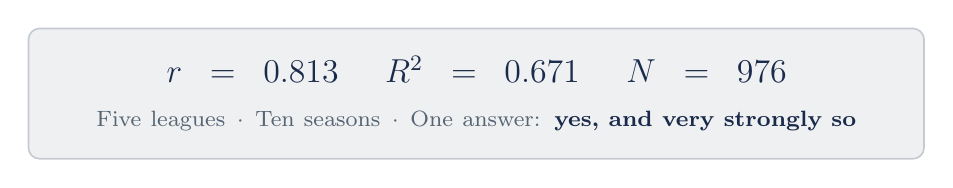
\begin{tikzpicture}
      \node[fill=NavyBlue!7, draw=NavyBlue!25, line width=0.6pt,
            rounded corners=4pt, inner sep=10pt,
            text width=0.88\linewidth, align=center]{%
        {\large\bfseries\color{NavyBlue}
          $r = 0.813$ \quad $R^2 = 0.671$ \quad $N = 976$}\\[4pt]
        {\footnotesize\color{SlateGrey}
          Five leagues\enspace$\cdot$\enspace
          Ten seasons\enspace$\cdot$\enspace
          One answer: \textbf{\color{NavyBlue}yes, and very strongly so}}
      };
    \end{tikzpicture}
  \end{center}
  \vspace{6pt}

  % ── Bottom: two columns ─────────────────────────────────────
  \begin{columns}[T]
    \begin{column}{0.48\textwidth}
      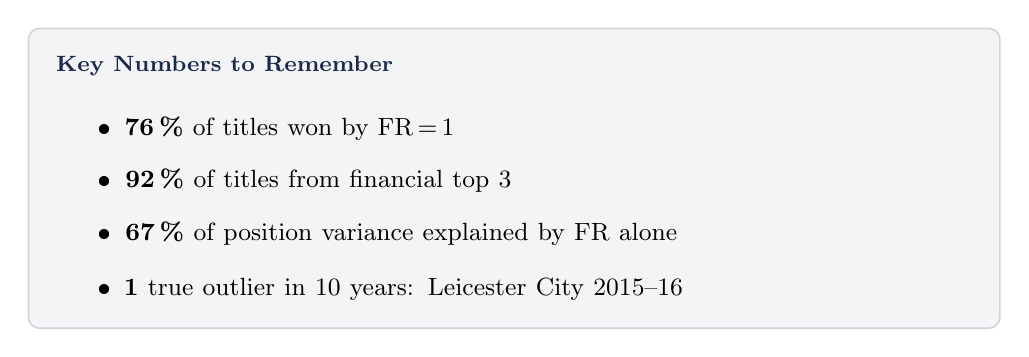
\begin{tikzpicture}
        \node[fill=NavyBlue!5, draw=NavyBlue!20, line width=0.6pt,
              rounded corners=4pt, inner sep=10pt,
              text width=\linewidth-14pt]{%
          {\footnotesize\bfseries\color{NavyBlue}Key Numbers to Remember}
          \vspace{4pt}
          \begin{itemize}\setlength\itemsep{4pt}
            {\small
            \item \textbf{76\,\%} of titles won by FR\,=\,1
            \item \textbf{92\,\%} of titles from financial top~3
            \item \textbf{67\,\%} of position variance explained
                  by FR alone
            \item \textbf{1} true outlier in 10 years:
                  Leicester City 2015--16
            }
          \end{itemize}
        };
      \end{tikzpicture}
    \end{column}
    \begin{column}{0.48\textwidth}
      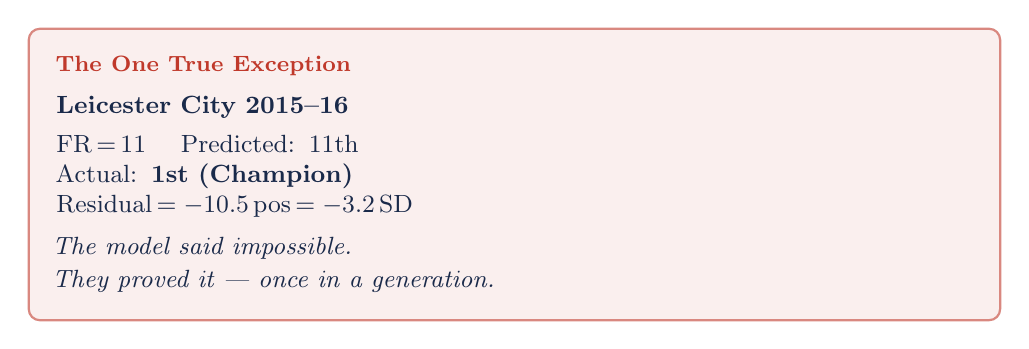
\begin{tikzpicture}
        \node[fill=AlertRed!8, draw=AlertRed!60, line width=0.8pt,
              rounded corners=4pt, inner sep=10pt,
              text width=\linewidth-14pt]{%
          {\footnotesize\bfseries\color{AlertRed}
            The One True Exception}\\[4pt]
          {\small\color{NavyBlue}
            \textbf{Leicester City 2015--16}\\[3pt]
            FR\,=\,11 \quad Predicted: 11th\\
            Actual: \textbf{1st (Champion)}\\
            Residual\,$= -10.5$\,pos\,$= -3.2$\,SD\\[4pt]
            \textit{The model said impossible.\\
            They proved it --- once in a generation.}}
        };
      \end{tikzpicture}
      \vspace{6pt}
      {\scriptsize\color{SlateGrey}
        \textbf{Data:} ESPN~FC + Transfermarkt\quad
        \textbf{Period:} 2015--16 to 2024--25\\
        \textbf{Models:} OLS (A--H, H2--H4), Logit (E)}
    \end{column}
  \end{columns}
\end{frame}

\end{document}
